El hombre, en su continua evolución, ha utilizado el lenguaje como una herramienta creadora de conocimiento transferible a sus congéneres o cualquier otro ser que interactuase con él. Con esto, “los humanos han desarrollado el lenguaje como un instrumento ligero y conveniente para mantener sus relaciones”\cite{dynamics}. 

En la comunicación entre congéneres, el lenguaje puede ser dividido en dos funciones: función de transmisión de información (gossip) y función de entendimiento del estado interno (estado mental) del congénere (mentalisation)\cite{dynamics}. Estas funciones de transmisión y entendimiento del otro han permitido que dos o varios humanos puedan asociarse entre sí formando redes sociales.

Las redes sociales no son otra cosa que la formación de lazos de algún tipo (emocional, de pertenencia a una comunidad, de trabajo, etc.) entre individuos que pueden ser organizaciones o humanos.\cite{sna_startups} En la figura \ref{fig:red_al_quaeda} puede verse cómo es representada la red social que forman las células terroristas de Al-Qaeda.

\begin{figure}[!htb]
  \begin{center}
    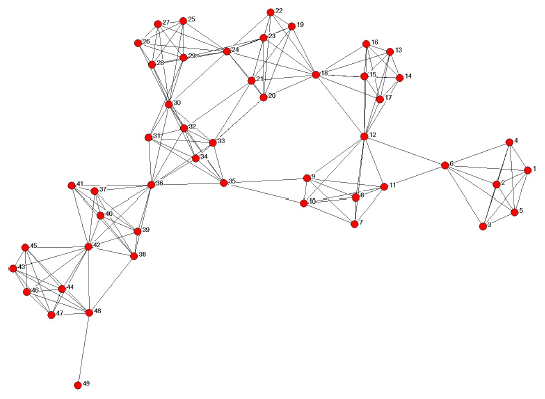
\includegraphics[width=11cm]{./imagenes/red_al_qaeda.png}
    \caption{Red social conformada por las células terroristas de Al-Qaeda.}
    \label{fig:red_al_quaeda}
  \end{center}
\end{figure}

La evolución de los servicios proporcionados a través de la internet ha sido drástica puesto que ha cambiado el modo de vida de las personas. En la figura \ref{fig:utilizacion_internet} se evidencia el crecimiento de la internet (de los servicios que en ella se soportan) se da en función de los servicios de conectividad social que son creados y soportados en ella. La web 1.0 fue utilizada en mayor medida por científicos para el intercambio de información en formato hipertexto. No había una interacción fuerte entre cada científico sino que ellos acudían a internet para buscar o poner a disposición material científico. Con la venida de la web 2.0 y la introducción de la interacción del usuario con la web generando contenido en tiempo real, así se crearon servicios de redes sociales en-línea (OSN en inglés: On-line Social Network), produciento una partición en los tipos de redes sociales. Así, las redes sociales a las que pertenece el ser humano en la era digital se dividieron convenientemente en “redes sociales fuera de línea” y redes sociales en línea (Offline Social Network y Online Social Network).

\begin{figure}[!htb]
  \begin{center}
    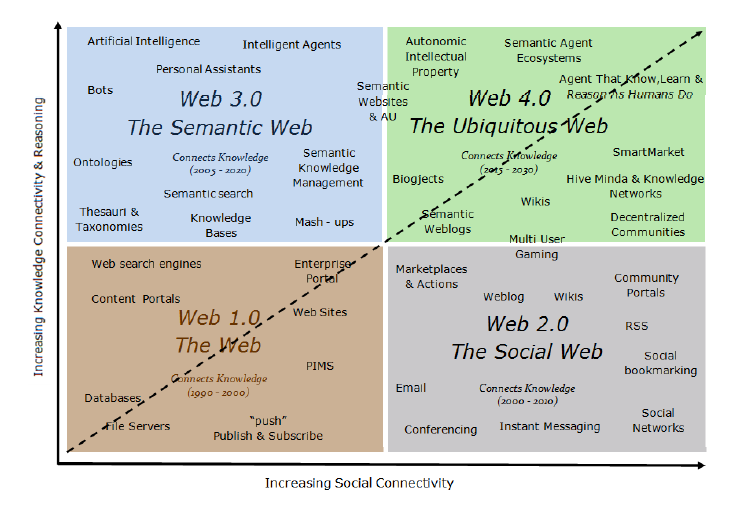
\includegraphics[width=11cm]{./imagenes/utilizacion_internet.png}
    \caption{Cambio de la utilización de internet en función de los servicios de conectividad social que son creados y soportados en ella}
    \label{fig:utilizacion_internet}
  \end{center}
\end{figure}

Las redes sociales fuera de línea son las redes sociales que se forman por comunicación tradicional (lenguaje oral y escrito en medios que difieran de aquellos que utilizan las telecomunicaciones). Las redes sociales en línea son aquellas redes sociales que están formadas por cibernautas y en las cuales la comunicación se da por medio de los servicios de redes sociales.

La administración de una red social fuera de línea fue estudiada desde inicios del siglo XX\cite{dynamics} con un enfoque socio-matemático llamado “análisis de redes sociales” (SNA por sus siglas en ingles: Social Network Analisis). Sin embargo, era difícil el análisis del comportamiento humano según los designios de la SNA puesto que la información debía ser recopilada por medio de entrevistas a las personas. Aún así, el enfoque SNA fue utilizado para analizar el comportamiento terrorista o inclusive el comportamiento de trabajadores en una empresa.\cite{sna_startups}

Con la creación de las OSN y la gran cantidad de información que describe el comportamiento humano sobre este tipo de red social, ha sido más sencillo utilizar el enfoque de la SNA para estudiar que comportamientos tienen los humanos sobre una red social establecida.

Los servicios de redes sociales (SNS por sus siglas en ingles: Social Network Services) como Facebook, LinkedIn, Twitter, SportTracker o Xportia, ofrecen servicios para la gestión de la OSN de cada usuario que acceda a estas aplicaciones. Según un estudio hecho para medir la experiencia de usuario (UX por sus siglas en ingles: User eXperience) en los SNS, se encontraron 8 categorías que son críticas a la hora de diseñar una SNS y son:

1. Self-expresion: Capacidad que tengan las OSN de compartir contenido relacionado a la vida real de los usuarios tal como lo pueden ser las fotos, los videos, los comentarios o las comunicaciones directas.
2. Reciprocity: Interacción bilateral en tiempo real, es decir, interacción instantánea con uno o varios individuales en la OSN (por ejemplo, por medio de los servicios de mensajería instantánea).
3. Learning: La información recibida por medio de la OSN debe poder ser utilizada en pro del desarrollo cognitivo del individual; debe existir información útil al individual que usa la OSN.
4. Curiosity: El contenido de la OSN debe ser interesante para quien la utiliza.
5. Suitability of functionality: Se refiere a cuán “utilizable” es una funcionalidad.
6. Suitability of content: La calidad y exactitud de la información que en la OSN reside debe ser suficiente para el individual perteneciente a ella.
7. Completeness of the user network: Los individuales deben querer pertenecer a la red social y buscar eficientemente a otros individuales para poder formar lazos con ellos y hacer crecer su red social.
8. Trust and privacy: Confianza en los servicios de las OSN, así como también la capacidad que tiene el usuario de gestionar la privacidad del contenido que comparte en dicha OSN.\cite{social_experience}

De acuerdo al enfoque SNA, las redes sociales pueden estar divididas en clusters, que no son más que agrupaciones de individuales sobre una red social por algún concepto como, por ejemplo, la pertenencia a una comunidad. Con lo anterior, podemos encontrar que algunos SNS ofrecen servicios para gestionar las OSN de sus usuarios centrándose en algún tipo de comunidad en específico y, la información que circula por ese tipo de comunidades, es diferente a la que pasa por SNS descentralizados (como Facebook y twitter). Viendo Facebook como una agrupación de clusters con temáticas tan diferentes como lo son los deportes y la música, la ciencia y la vida cotidiana, se puede decir que algunos SNS se enfocan en alguna de estas temáticas. En este caso, el cluster o temática que compete al trabajo a elaborar es el deporte.

Es posible hacer una división del cluster deporte en otros subclusters de cada uno de los deportes que existen en el mundo o en la clasificación de los deportes que han dado organizaciones como, por ejemplo, la IWGA (Internation WorldGames Association). Lo que se quiere con este trabajo es aportar al crecimiento de las redes sociales fuera de linea de las personas que practiquen deporte sin importar si lo hacen a nivel profesional o aficionado por medio de un SNS orientado a los deportes en general y, por lo tanto, el cluster que se ha escogido para trabajar es el del deporte como cluster mismo.

Se investigó acerca de las redes sociales existentes enfocadas a la temática del deporte y se encontró que muchas de ellas son utilizadas en mayor medida en España y que todas ellas están soportadas sobre tecnologías web. En general, solo se encontraron dos redes sociales deportivas orientadas a cualquier deporte asociadas a aplicaciones para smartphones disponibles en el la tienda virtual de Android o en la tienda virtual de Apple (La red social de Fitivity y Huddlers).

Así, con la evolución de la comunicación humana trasladándose a los espacios virtuales por medio de las OSN y la falta de aplicaciones, en el campo de los smartphones, que soporten interacciones sociales enfocadas a los deportes en general, en este trabajo se creará un SNS centrado en los deportes sobre tecnologías Android para la administración de las OSN de cada persona en un ámbito deportivo desde su dispositivo móvil.
